\documentclass[../main.tex]{subfiles}

\begin{document}
\begin{problema}[4]
	Se derivará la ecuación de equilibrio de una placa. Para ello,
	considerar una placa, de material Hookeano, que sufre una deformación
	longitudinal, donde el único esfuerzo sobre la placa es de extensión
	al aplicar una distribución de esfuerzos en sus extremos izquierdo y derecho,
	como se muestra  en la \zcref{fig:placa-p1}. Considerar que no hay fuerzas de
	cuerpo y que la placa tiene un ancho \(h\), un largo \(L\) y el
	grosor es pequeño en la dirección \(z\).

	\begin{enumerate}
		\item ¿Qué condiciones de frontera debe cumplir el tensor de
		      esfuerzos \(\dbloverline{\sigma}\) en \(z = \pm \tfrac{h}{2}\)?
		\item Considerando que la placa es delgada se puede decir
		      que \(\sigma_{zx} = \sigma_{zy} = \sigma_{zz} \simeq 0\) en
		      toda la placa. A partir de la relación constitutiva Hookeana
		      para \(\dbloverline{\sigma}\), escrita en términos de los
		      coeficientes de Lamé, \(\lambda\) y \(\mu\), obtener \(E_{zz}\)
		      como función de las componentes \(E_{xx}\) y \( E_{yy}\) del
		      tensor de deformaciones infinitesimales de Cauchy \(\dbloverline{E}\).
		\item Reescribir \(E_{zz}\) en términos de la razón de Poisson \(\nu\) y
		      no en términos de \(\lambda\) y \(\mu\), i.e. mostrar que
		      \(\tfrac{-\lambda}{\lambda + 2\mu} = \tfrac{\nu}{\nu - 1}\).
		\item A partir de la relación constitutiva Hookeana para \(\dbloverline{E}\),
		      escrita en términos de \(\nu\) y del módulo de Young \(Y\), encontrar las
		      componentes del tensor de deformaciones \(E_{xz}\) y \(E_{yz}\) y
		      mostrar que son nulos.
		\item  A partir de la relación constitutiva Hookeana para \(\dbloverline{\sigma}\),
		      escrita en términos de \(\nu\) y \(Y\), encontrar las componentes del
		      tensor de esfuerzos \(\sigma_{xy}, \sigma_{xx}\) y \(\sigma_{yy}\) como
		      funciones de las componentes del tensor de deformaciones
		      \(E_{xx}, E_{yy}\) y \(E_{xy}\). Usar la relación encontrada para
		      \(E_{zz}\) en el inciso (c).
		\item A partir de considerar que la placa está en equilibrio,
		      \(\nabla \cdot{\dbloverline{\sigma}} = 0\), se obtiene el
		      siguiente sistema de ecuaciones:

		      \begin{align*}
			      \pdv{\sigma_{xx}}{x} + \pdv{\sigma_{xy}}{y} & = 0, \\
			      \pdv{\sigma_{xy}}{x} + \pdv{\sigma_{yy}}{y} & = 0.
		      \end{align*}

		      Integrar ambas ecuaciones con respecto a \(z\) de \(-\tfrac{h}{2}\) a
		      \(\tfrac{h}{2}\). Escribir el resultado sin eliminar
		      el término \(h\).
		\item Reescribir el resultado de las integrales del inciso (f) en
		      términos de las componentes del vector de desplazamiento \(u_{x}\) y
		      \(u_{y}\), usando la relación entre \(\dbloverline{E}\) y \(\vect{u}\).
		      El resultado debe mostrar que la ecuación de equilibrio de la
		      placa es

		      \begin{equation*}
			      hY \Biggl[\dfrac{1}{1 - \nu^{2}}\nabla{\Bigl(\nabla \cdot{\vect{u}}\Bigr)} - \dfrac{1}{2(1 + \nu)}\nabla \mul{\Bigl(\nabla \mul{\vect{u}}\Bigr)}\Biggr] = 0,
		      \end{equation*}

		      tomando \(\nabla\) para 2D. Considerar que como la placa es
		      delgada, el vector de desplazamiento se puede aproximar como
		      \(\vect{u} \simeq u_{x}(x,y) \uvec{e}_{x} + u_{y}(x, y)\uvec{e}_{y}\).

		      Obsérvese que, cuando hay fuerzas de cuerpo \(\vect{f}\), la ecuación
		      de equilibrio de la placa es

		      \begin{equation*}
			      hY \Biggl[\dfrac{1}{1 - \nu^{2}}\nabla{\Bigl(\nabla \cdot{\vect{u}}\Bigr)} - \dfrac{1}{2(1 + \nu)}\nabla \mul{\Bigl(\nabla \mul{\vect{u}}\Bigr)}\Biggr] + \vect{P} = 0,
		      \end{equation*}

		      donde \(\vect{P} = \int \odif[sep-end=\medspace]{z} \vect{f}\).

		      Esta última ecuación no se tiene que derivar, solo es una observación
		      que servirá para el Ejercicio 2.

		      \begin{figure}[htb]
			      \centering
			      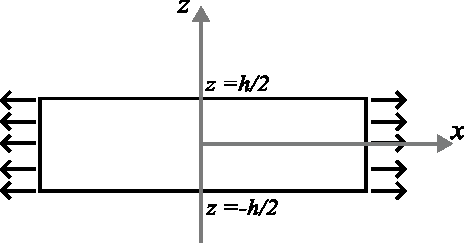
\includegraphics{figs/problema01.pdf}
			      \caption{Diagrama de una placa para el problema 1.}
			      \label{fig:placa-p1}
		      \end{figure}
	\end{enumerate}
\end{problema}
\end{document}
